\documentclass[prd,aps,twocolumn,a4paper,showkeys,nofootinbib]{revtex4-1}

\usepackage{amsmath}
\usepackage{amsfonts}
\usepackage{amssymb}	
\usepackage{graphicx}
\usepackage{color}
\usepackage[hidelinks]{hyperref}
\allowdisplaybreaks

\def\TODO{\textcolor{red}{TODO:}}
\def\Mc{{\cal M}_c}
\def\N{{\cal N}}
\def\M{{\cal M}}
\def\P{{\cal P}}
\def\Ix{{I_{\bar{x}}}}
\def\Iy{{I_y}}

\begin{document}
	
\title{Statistical errors}

\author{Simone Albanesi}

\date{\today}

\maketitle

%==========================================================
\section{Task}
%========================================================== 
The goal of this notes is to show how we can estimate the error/confidence interval
of a certain recovery/prediction.
The problem can be formulated as follows.
Consider a vector of variables $y$. Then we apply a certain transformation $\N$ so
that we have a new array of variables $s = \N(y)$. Then we construct
a new transformation $\M$ that satisfies $x=\M(s) = \M(\N(y))$ where
 $x$ is closest as possible to $y$. If $N$ is invertible, then the task is trivial
since $\M=\N^{-1}$ and thus $x=y$. However in general $\N$ is not invertible and we have to
rely on some heuristics to find $\M$, and the equality $x=y$ is not guaranteed. 
In other words, $x$ is an estimate of $y$ that we can obtain knowing $s=\N(y)$ and $\M$, 
and we want to estimate the error on $x$ using a statistical approach.
In our specific case, $y$ are the injected value, $N$ is the noise introduced by \texttt{GstLAL},
$s$ are the recovered quantities, $\M$ is a ML algorithm and thus $x$ are the predictions of our
ML algorithm. The expression $x \simeq y$ can be formalized requiring that $x$ minimize a loss 
function. To compute the error on the prediction $x$, we need to know the distribution 
of $y$ values at fixed $x$, namely $f_x(y)$. Then, from $f_x(y)$ we can compute the
confidence interval of the prediction $x$ and we are done. 
Note that if $\M$ is a smooth 1-dimensional function, then $f_x(y)$ would be a Dirac-delta. 
However, even in the 1d case, it could be argued that if $\M$ 
is not smooth, then is possible that in an 
arbitrarily small neighborhood of a certain $x$ we can have many different $y$ values. The elegant example 
is a self-similar function, the more realistic case is a non-continuous function with a lot of discontinuities.
In any case, if we are considering a ML algorithm, $\M$ should be smooth.
Fortunately, we are not working on a 1d problem, i.e. $x$ and $y$ are actually vectors,
so that if we consider one component at a time, for each $x_i$ value we can have many $y_i$. 
More precisely,we project
$\M^i(s_1, s_2,\dots,s_i,\dots)=(x_1,x_2,\dots,x_i,\dots)$ on the $(x^i,y^i)$ plane, so that
for each value of $x_i$ we can have different values of $y_i$ and thus $f_{x_i}(y_i)$ is not ill-posed. 
Treating each element of the arrays (features) separately means that we assume that the error associate to 
$x^i$ can be determined knowing only the $y^i$ distribution. 
Note that this is not equivalent to state that the error on $x^i$ depends only on $x^i$ itself, 
but it is quite the opposite, as discussed above.
In the following we drop the $i$-index on the features.

\section{Approach n.1: $\mu(x)$ , $\sigma(x)$, $\gamma(x)$ fits}
We can then consider the $(x,y)$ plane and define the sets
$\Ix = \{ x \in (\bar{x}-\frac{\Delta x}{2}, \bar{x}+\frac{\Delta x}{2}) \}$ and
$I_y^0 = \{y: \M\circ \N(y)\in I_{\bar{x}} \}$. Assuming $N$ large enough, we can consider a small $\Delta x$ 
and still have many elements in the sets $\Ix$ and $I_y^0$. We are interested in estimating the $y$-distribution
given a certain $x$, but what we are doing here is to consider many $y$ values that correspond to different
$x$ values. Therefore we introduce a linear transformation $\P_y: y \rightarrow y'=y+\bar{x}-x$ 
that defines a new set $\Iy = \{ \P_y(y), y\in I_y^0 \}$. Note that the transformation 
$P: (x,y)\rightarrow (\bar{x}, y')$ is a translation of the $(x,y)$ point along the identity line $y=x$.
We thus find a set of $y$ values that correspond to an unique $x$ value, $\bar{x}$.
The distribution of $y$ values will give us information on the accuracy of our transformation 
$\M\circ\N$ for the considered feature, since they are all the values that can be predicted for a certain value $x$. 
This last sentence can sound strange since $\M$ is a function and thus should predict a single value for each $x$. 
However, as discussed above, consider that we are actually considering the projection of $\M\circ\N$ in the $(x,y)$.
We say that $\Ix$ and $\Iy$ define a {\it bin}. To cover all the possible values of $x$, we build many bins.
For each bin we want to determine $f_{\bar{x}}(y)$. 

We assume that $f_{\bar{x}}(y)$ can be written analytically as a skewed normal Gaussian distribution.
This 1-parameter family of continuously-deformed Gaussian distributions depends on three parameters: the location $\xi$, 
the scale $\omega$, and the shape $\alpha$. If $\alpha=0$ then the location is the mean value, the scale 
is the standard deviation and we recover the Gaussian distribution.
These three parameters can reconstructed analytically for each bin computing the mean $\mu$, variance $\sigma^2$, and 
skewness $\gamma$ of the points in $\Iy$. 
Consider that in order to do the transformation $(\mu,\sigma,\gamma)\rightarrow(\xi,\omega,\alpha)$, the
skewness should be in the interval $(-1,1)$, so that if we measure $|\gamma|>0.99$, we set $\gamma=\pm 0.99$.
After the computation of $(\mu,\sigma,\gamma)$ for each bin, we do a polynomial fit in order to obtain 
$(\mu(x),\sigma(x),\gamma(x))$. If the fit is good, then for each value of $x$ we can obtain $f_{\bar{x}}(y)$
and we are done. 

Summary:
\begin{enumerate}
	\item Build the bins $(\Ix,\Iy)$ for many $\bar{x}$ so that we cover the whole parameter space;
	\item for each bin we compute the distribution moments $(\mu,\sigma,\gamma)$ on $\Iy$;
	\item we fit the moments found in order to obtain $(\mu(x),\sigma(x),\gamma(x))$;
	\item from a value $x^*$ we can obtain $(\mu(x^*),\sigma(x^*),\gamma(x^*))$ and 
	compute $(\xi, \omega, \alpha)$, i.e. $f_{x^*}(y)$.
\end{enumerate}

The problem with this method is that the fits used to obtain the momenta must be good and this strongly depends
on the distribution of data in the parameter space. This method works for $m_1$ and $m_2$ on the dataset with
only nonspinning BNS, see Fig.~\ref{fig:approach1_BNS}, but does not work for the complete dataset.
One could try to improve the bin-sampling, but I have no practical ideas on how to do that. 

\begin{figure*}[t]
	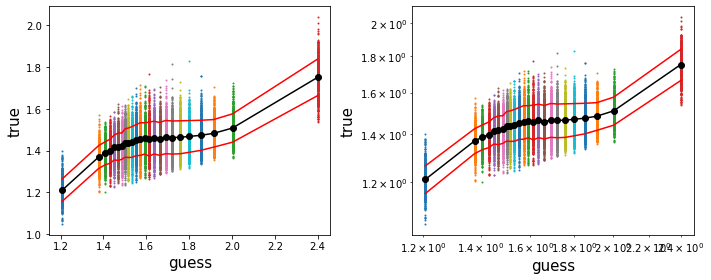
\includegraphics[width=0.45\textwidth]{./FigsErr/v1_BNS_rec_m1_bins.png}
	\hspace{0.8cm}
	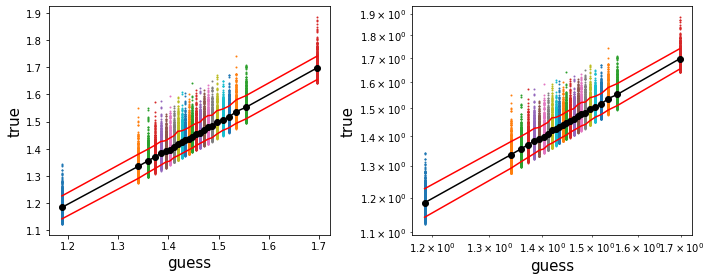
\includegraphics[width=0.45\textwidth]{./FigsErr/v1_BNS_pred_m1_bins.png} \\
	
	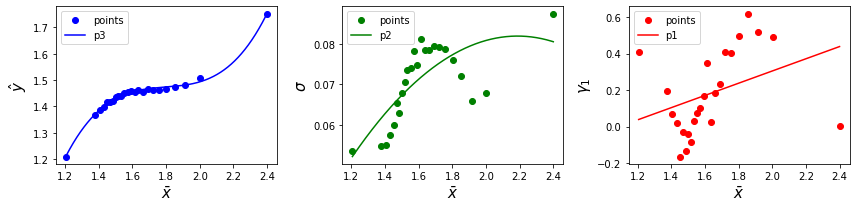
\includegraphics[width=0.45\textwidth]{./FigsErr/v1_BNS_rec_m1_fits.png}
	\hspace{0.8cm}
	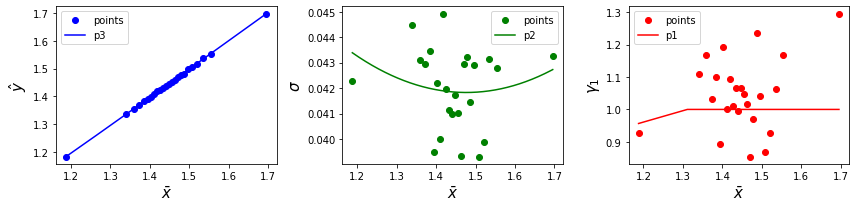
\includegraphics[width=0.45\textwidth]{./FigsErr/v1_BNS_pred_m1_fits.png} \\
	
	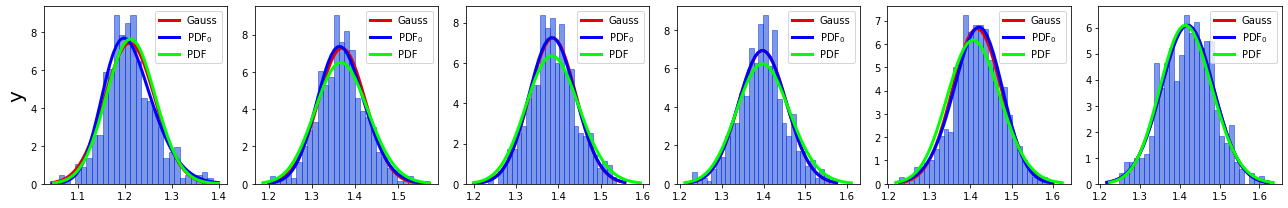
\includegraphics[width=0.45\textwidth]{./FigsErr/v1_BNS_rec_m1_distr1.png}
	\hspace{0.8cm}
	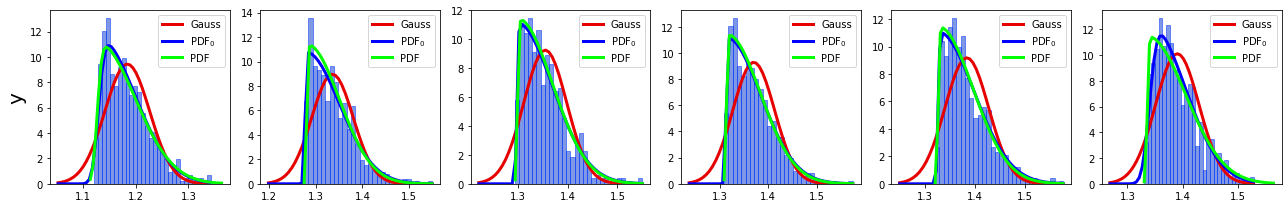
\includegraphics[width=0.45\textwidth]{./FigsErr/v1_BNS_pred_m1_distr1.png} \\
	
	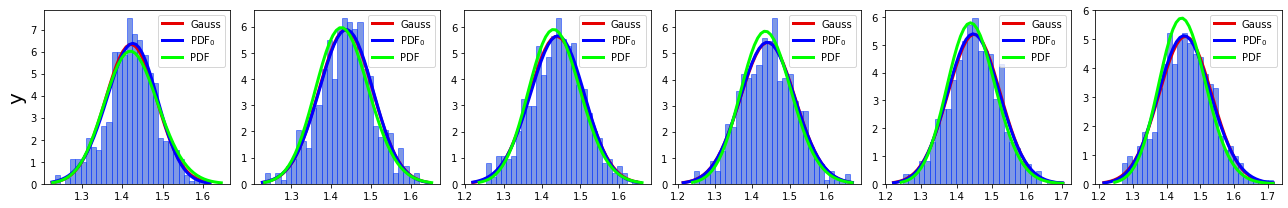
\includegraphics[width=0.45\textwidth]{./FigsErr/v1_BNS_rec_m1_distr2.png}
	\hspace{0.8cm}
	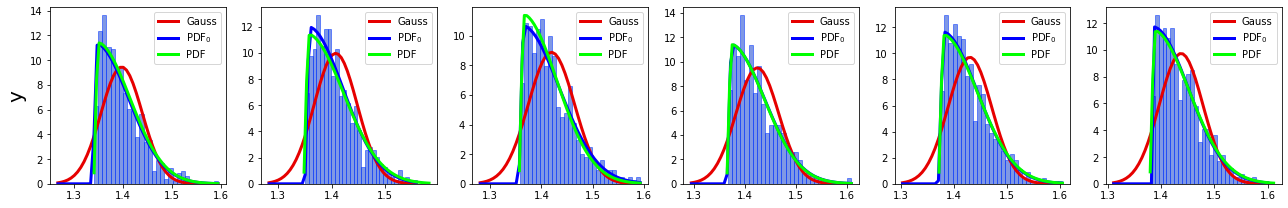
\includegraphics[width=0.45\textwidth]{./FigsErr/v1_BNS_pred_m1_distr2.png} \\
	
	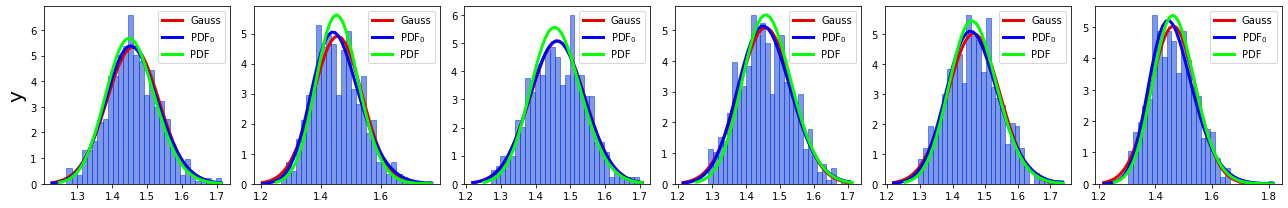
\includegraphics[width=0.45\textwidth]{./FigsErr/v1_BNS_rec_m1_distr3.png}
	\hspace{0.8cm}
	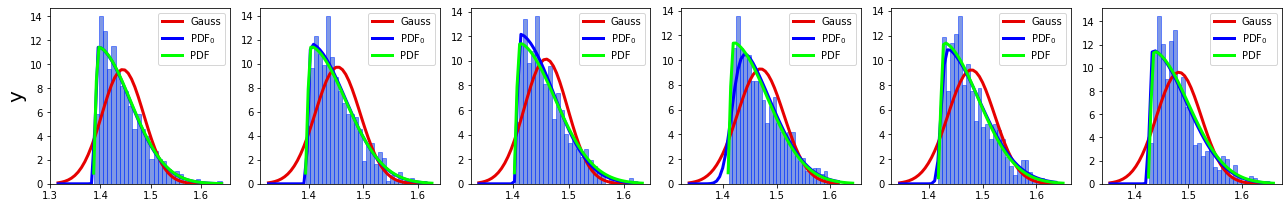
\includegraphics[width=0.45\textwidth]{./FigsErr/v1_BNS_pred_m1_distr3.png} \\
	
	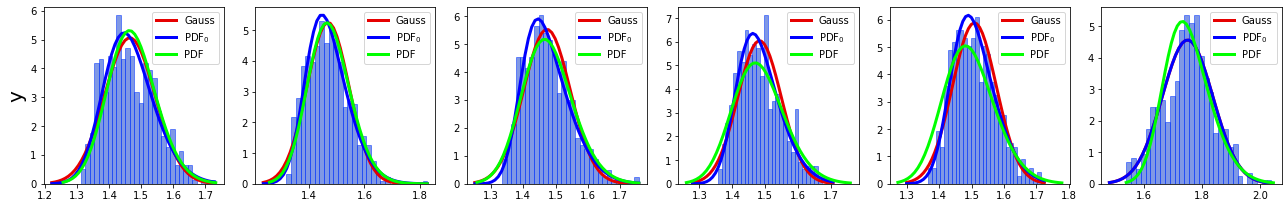
\includegraphics[width=0.45\textwidth]{./FigsErr/v1_BNS_rec_m1_distr4.png}
	\hspace{0.8cm}
	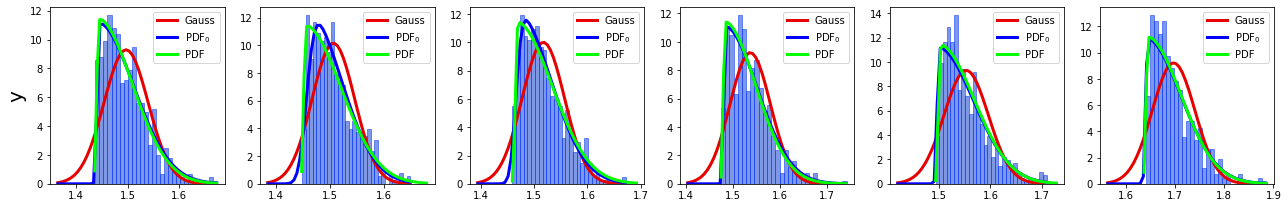
\includegraphics[width=0.45\textwidth]{./FigsErr/v1_BNS_pred_m1_distr4.png} 
	\caption{\label{fig:approach1_BNS} Method 1 applied to recovered (left) and predicted (right) $m_1$ for the 
		nonspinning BNS dataset. To build the histograms and thus the PDFs, we consider $n\simeq 565$ points and only 
		the $y$ values that are included in the 5 $\sigma$ interval. The orders of polynomials
		used for $(\mu,\sigma,\gamma)$ are 3, 2, and 1, respectively (with $\gamma_{\rm max}=0.99$).
		The green curve is the one computed 
		from the fits, while the blue one is obtained directly from $\Iy$. The red one is computed from $\Iy$ 
		under Gaussian-hypothesis. }
\end{figure*}


\end{document}